% TU Delft Beamer template
% Author: Maarten Abbink
% Delft University of Technology
% March 2014
% Version 2.0
% Based on original version 1.0 of Carl Schneider
\documentclass{beamer}
\usepackage[english]{babel}
\usepackage{calc}
\usepackage[absolute,overlay]{textpos}

\mode<presentation>{\usetheme{default} \usecolortheme{seahorse}}

\title[BEP]{Virtual Asssitant Web App\\ \small{Bachelor Thesis}}
%\subtitle
\institute[TU Delft]{Delft University of Technology}
\author{A. Hambenne\\
S. Jahanshahi}
\date{\today}

% Insert frame before each subsection (requires 2 latex runs)
\AtBeginSubsection[] {
	\begin{frame}<beamer>\frametitle{\titleSubsec}
		\tableofcontents[currentsection,currentsubsection]  % Generation of the Table of Contents
	\end{frame}
}	


% define a symbol which can be removed if you don't need it
\newcommand{\field}[1]{\mathbb{#1}}
\newcommand{\Zset}{\field{Z}}

\begin{document}

{
% remove the next line if you don't want a background image
\usebackgroundtemplate{
\includegraphics[width=\paperwidth,height=\paperheight]{images/background-titlepage.jpg}}%
\setbeamertemplate{footline}{\usebeamertemplate*{minimal footline}}
\frame{\titlepage}
}

{\setbeamertemplate{footline}{\usebeamertemplate*{minimal footline}}
% \begin{frame}\frametitle{\titleTOC}
% 	\tableofcontents
% \end{frame}
}



%What's about

\begin{frame}
\frametitle{What's it about?}
\centering

\includegraphics[scale=0.16]{./images/va.png}
\end{frame}

%Outline
\begin{frame}\frametitle{Outline}
	\begin{itemize}
		\item Research 
		\item Set-up
		\item Technologies
		\item Design Architecture
		\item Features
		\item Metrics  \& Evaluation
		\item Demo
		\item Q\&A Session
	\end{itemize}
\end{frame}

%Research-Analysis
\begin{frame}\frametitle{Research}\framesubtitle{Analysis }
\begin{itemize}
	\item Domain analysis : the problem, project stakeholders
	\item Defining client requirement: interview , meetings with project owner, etc
	\item Translating : Client wishes to functional \& technical requirements
	\item Benchmarking : Framework, Methodologies, programming languages
\end{itemize}
	
\end{frame}
%Research-SETUP
\begin{frame}\frametitle{Set up}
\begin{itemize}
	\item Scrum team: roles, sprint meeting, etc
	\item Tools installation: Framework, editors, libraries 
	\item Organization : Trello 
	\item Project: Continuous integration , planning 
	\item control version: Github
\end{itemize}
	
\end{frame}

%Technologies
\begin{frame}
\frametitle{Technologies}
\centering

\includegraphics[scale=0.37]{./images/presentation_techlogos.png}
\end{frame}
%Design1-MVC
\begin{frame}
\frametitle{Design}\framesubtitle{Model View Controller}
\centering
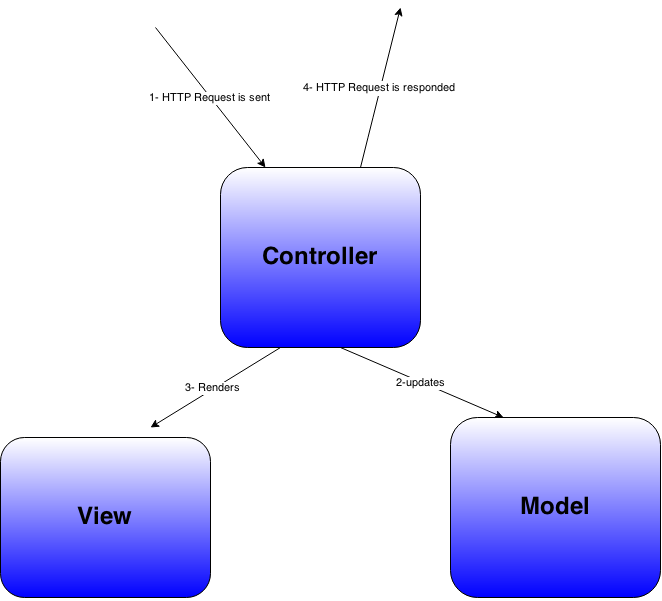
\includegraphics[scale=0.26]{./images/MVCdiag.png}
\end{frame}
%Design1-rma

\begin{frame}
\frametitle{Design}\framesubtitle{Relational Model}
\centering
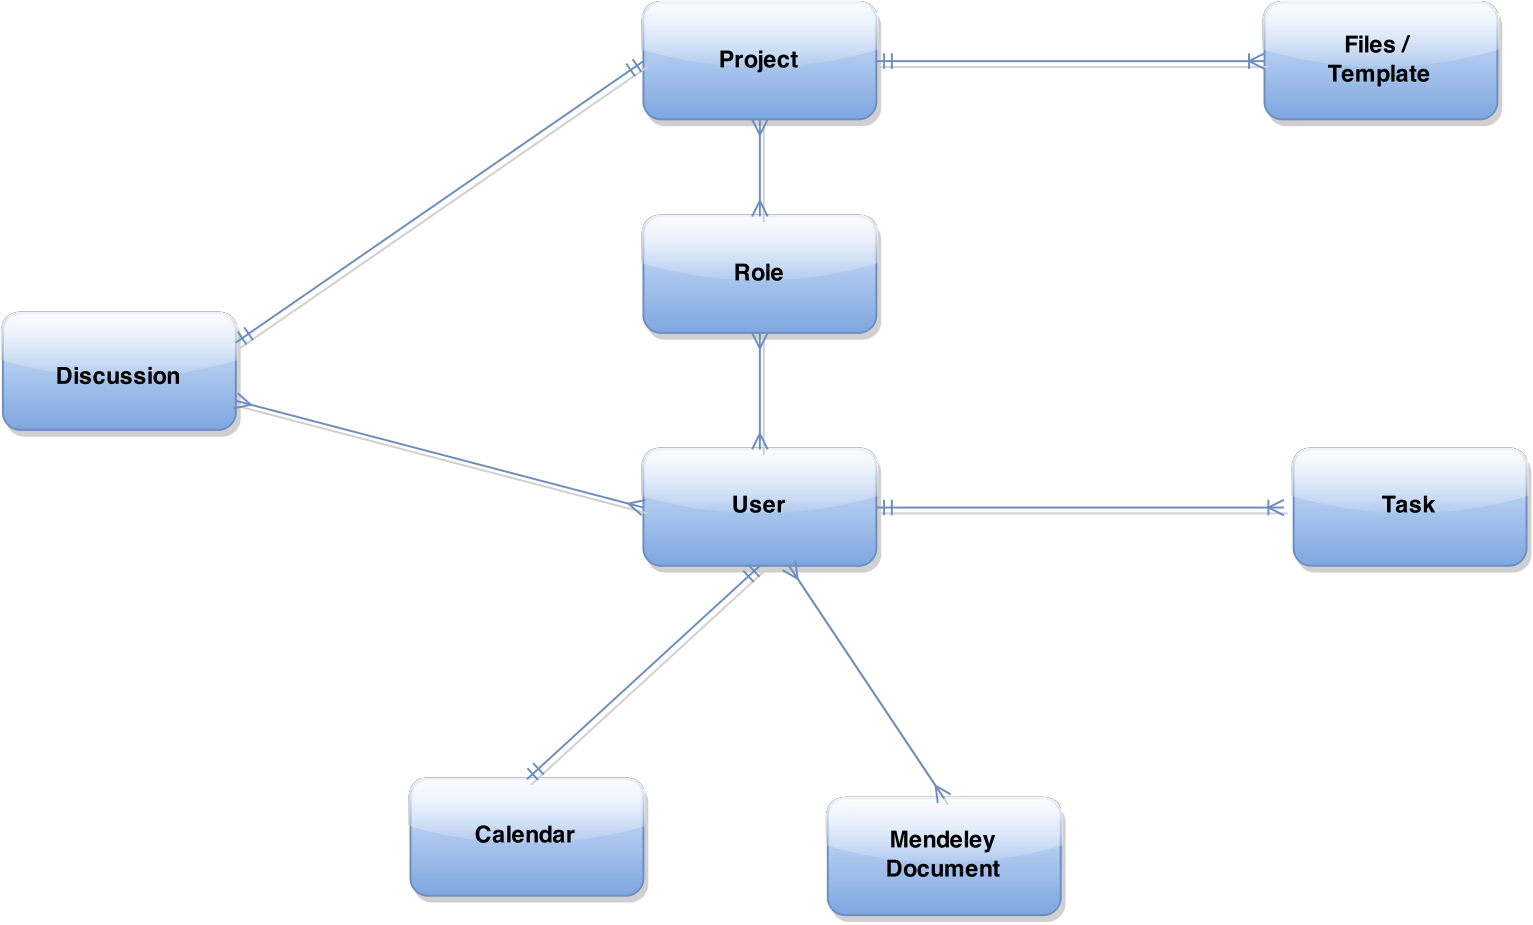
\includegraphics[scale=0.2]{./images/RMA.png}
\end{frame}

%Calendar
\begin{frame}
\frametitle{}\framesubtitle{}
	\begin{itemize}
		\item helps researchers make planning for their project 
		\item Asynchronous(no need to refresh the page)
		\item Re-sizable, Drag-able, Instant update
		\item Sorted list of event(ascending) 
	\end{itemize}
\end{frame}


%OAUTH2
\begin{frame}
\frametitle{Features}
\framesubtitle{OAuth2 Authentication}
	\begin{itemize}
		\item External authentication
		\item Google Plus and Mendeley
		\item Existing Google Plus OAuth2 library
		\item Extended library for Mendeley
		\item Support for Facebook, Twitter, GitHub,...
	\end{itemize}
\end{frame}

%PROJECT
\begin{frame}
\frametitle{Features}
\framesubtitle{Projects}
	\begin{itemize}
		\item Create and join
		\item Three roles: Owner, Reviewer and Guest
		\item Predefined template vs. own template
		\item Owners and reviewers can upload, every member can download
		\item Invitation-only (By Owner)
	\end{itemize}
\end{frame}

%DISCUSSION
\begin{frame}
\frametitle{Features}
\framesubtitle{Discussions}
	\begin{itemize}
		\item Multiple discussions per project
		\item Visible and accessible to every member
		\item Chat-like (AngularJS)
		\item One top-comment with sub-comments
	\end{itemize}
\end{frame}

%TASKS
\begin{frame}
\frametitle{Features}
\framesubtitle{Tasks}
	\begin{itemize}
		\item User specific
		\item Personal
		\item Due date and description
		\item Done or To-Do
		\item Can be deleted and redone
	\end{itemize}
\end{frame}

%MENDELEY LIBRARY SHARING
\begin{frame}
\frametitle{Features}
\framesubtitle{Mendeley Library Sharing}
	\begin{itemize}
		\item Link and Sync Mendeley Library
		\item Uses metadata (Title, Authors, Type,...)
		\item Mendeley OAuth2 API
		\item Global feature
	\end{itemize}
\end{frame}

%FORM VALIDATION
\begin{frame}
\frametitle{Security}
\framesubtitle{Form Validation}
	\begin{itemize}
		\item Verified users exclusive
		\item Session validation per action
		\item REGEX expressions
	\end{itemize}
\end{frame}

%METRICS 1
\begin{frame}
\frametitle{Metrics \& Evaluation}
\framesubtitle{GitHub \& Code}
	\begin{figure}
		
\includegraphics[scale=0.3]{./images/github_stats.png}
		\caption{GitHub Statistics}
	\end{figure}
	\begin{itemize}
		\item Total lines of code: \textbf{5341} (including statically imported plugins)
		\item Total code coverage: \textbf{69\%}
	\end{itemize}
\end{frame}

%METRICS 1 (BIS)
\begin{frame}
\frametitle{Metrics \& Evaluation}
\framesubtitle{GitHub \& Code}
	\begin{figure}
		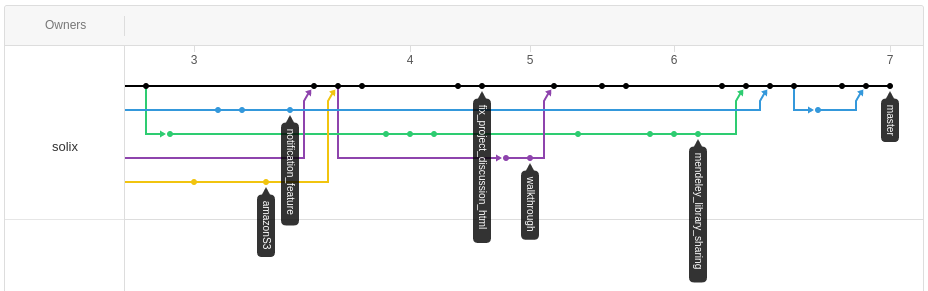
\includegraphics[scale=0.3]{./images/github_tree.png}
		\caption{GitHub Branching Tree}
	\end{figure}
\end{frame}

%METRICS 2
\begin{frame}
\frametitle{Metrics \& Evaluation}
\framesubtitle{Scrum}
	\begin{itemize}
	 \item \textbf{12} Sprints in \textbf{14} weeks
	 \item 
	\end{itemize}
\end{frame}

%SELF-EVALUATION: WHAT WENT WRONG
\begin{frame}
\frametitle{Metrics \& Evaluation}
\framesubtitle{Self-evaluation: The bad parts}
	\begin{itemize}
	 \item Agreeing before implementing
	 \item Timeline buffer zones
	 \item Optimal < Functional
	 \item Unverified Mendeley just works
	\end{itemize}
\end{frame}

%SELF-EVALUATION: WHAT WENT RIGHT
\begin{frame}
\frametitle{Metrics \& Evaluation}
\framesubtitle{Self-evaluation: The good parts}
	\begin{itemize}
	 \item Front-end first, then backend
	 \item Practicality < Durability
	\end{itemize}
\end{frame}

%SELF-EVALUATION: IMPORTANT LESSONS
\begin{frame}
\frametitle{Metrics \& Evaluation}
\framesubtitle{Self-evaluation: What we learned}
	\begin{itemize}
	 \item Be realistic
	 \item Choose tools wisely
	 \item Use of multiple technologies combined
	\end{itemize}
\end{frame}

%Demo time
\begin{frame}
\frametitle{Demo Time!}
\framesubtitle{beta version}


\begin{columns}
\column{0.7\textwidth}
\begin{itemize}
	\item We need 3 volunteers 
	\item \url{intense-stream-5056.heroku.com}
	
\end{itemize}\column{0.3\textwidth}
\begin{figure}%[2]
    \centering
    \href{intense-stream-5056.heroku.com}{
\includegraphics[scale=0.5]{./images/beta.png}}
\end{figure}		
\end{columns}

\end{frame}


\end{document}
